\documentclass[11pt]{article} 

\usepackage{deauthor,times,graphicx}
\usepackage{url}
\usepackage{subfig}

%\graphicspath{{authorname/}}

%\newcommand{\reffig}[1]{Figure~\ref{fig:#1}}
%\newcommand{\refsec}[1]{Section~\ref{sec:#1}}
%\newcommand{\reftab}[1]{Table~\ref{tab:#1}}

\begin{document}

\newcommand{\reffig}[1]{Figure~\ref{fig:#1}}
\newcommand{\refsec}[1]{Section~\ref{sec:#1}}
\newcommand{\reftab}[1]{Table~\ref{tab:#1}}

\title{Scheduling Data-Intensive Tasks on Heterogeneous Many Cores}

\author{P{\i}nar T\"oz\"un \\ IT University of Copenhagen \\ \texttt{pito@itu.dk}
\and Helena Kotthaus \\ TU Dortmund University \\ \texttt{helena.kotthaus@tu-dortmund.de}}

\maketitle

\begin{abstract}

Scheduling various data-intensive tasks over the processing units of a server
has been a heavily studied but still challenging effort.
In order to utilize modern multicore servers well,
a good scheduling mechanism has to be conscious of different dimensions of parallelism offered by these servers.
%both the vertical and horizontal parallelism offered by these servers.
This requires being aware of the micro-architectural features of processors,
the hardware topology connecting the processing units of a server,
and the characteristics of these units as well as the data-intensive tasks.
The increasing levels of parallelism and heterogeneity in emerging server hardware
amplify these challenges in addition to the increasing variety of data-intensive applications.

This article first surveys the existing scheduling mechanisms targeting
the utilization of a multicore server with uniform processing units. 
Then, it revisits them in the context of emerging server hardware composed of many diverse cores
and identifies the main challenges.
Finally, it concludes with the description of a preliminary framework targeting these challenges.
Even though this article focuses on data-intensive applications on a single server,
many of the challenges and opportunities identified here are not unique to such a setup,
and would be relevant to other complex software systems as well as
resource-constrained or large-scale hardware platforms. 

\end{abstract}

\section{Introduction}
\label{sec:intro}

% why scheduling
Utilizing the processors of commodity servers well is crucial to avoid wasting
resources, energy, and money in data centers regardless of their scale \cite{Hamilton10}.
As a result, quest to remove the bottlenecks of data management systems causing underutilization
of modern commodity servers have been the focus of many past and ongoing work \cite{AilamakiLTPP17}.
One of the essential challenges in this quest is scheduling various data-intensive tasks
effectively over the processing units that are available to these tasks. 
The fundamental evolution of the server hardware and the increasing variety
of the data-intensive applications over the recent years amplify this challenge.

\begin{figure}
\subfloat[\label{fig:hw}]{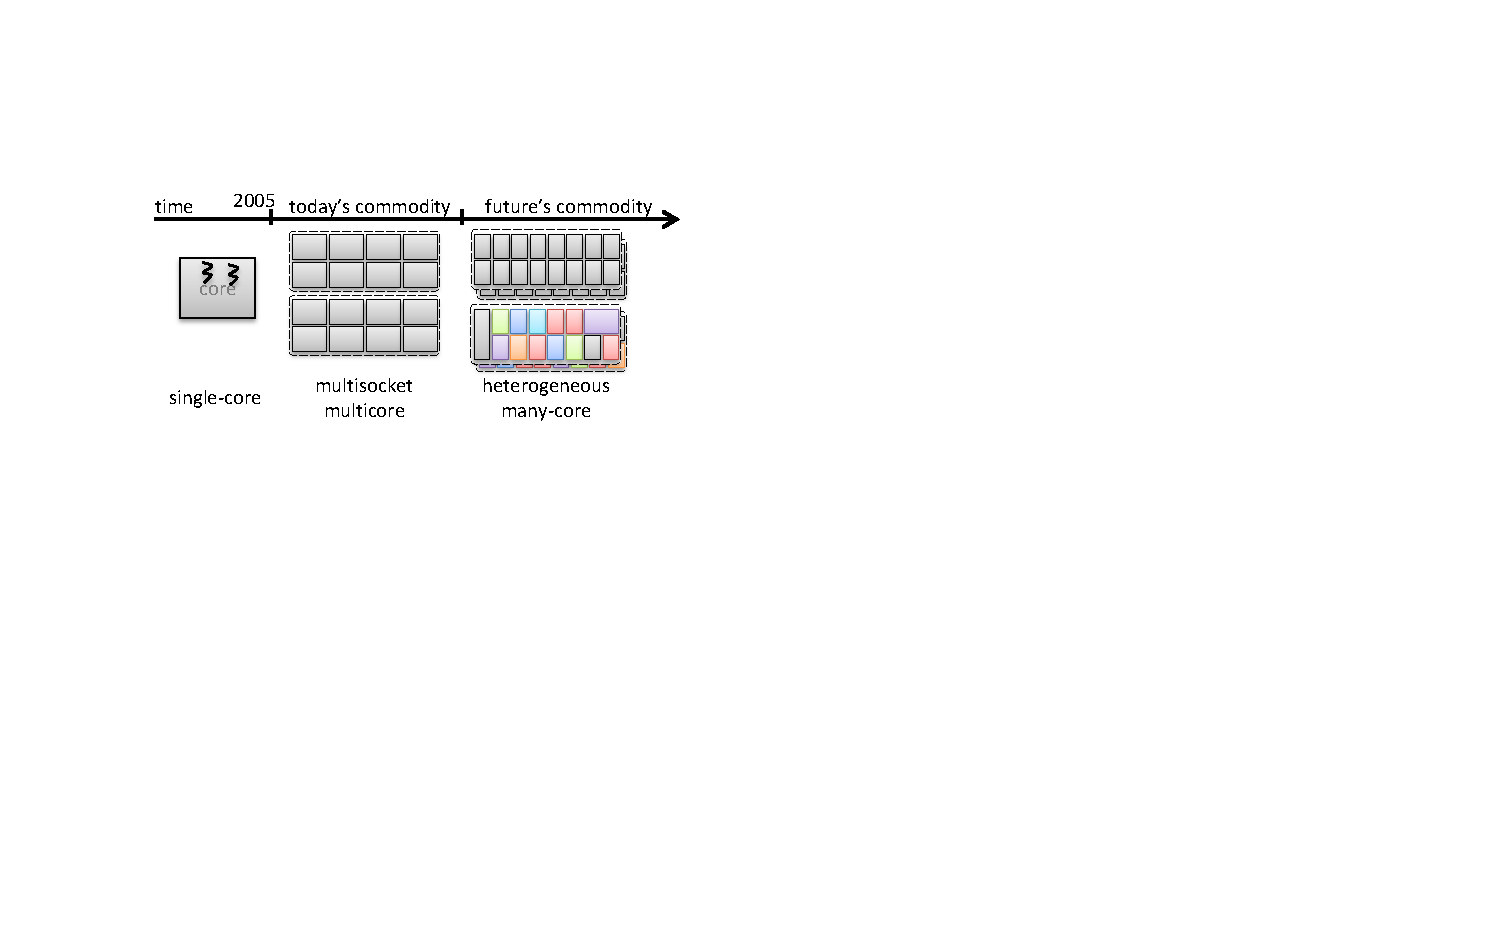
\includegraphics[width=0.6\textwidth]{fig-hw.pdf}}
\hfill
\subfloat[\label{fig:dia}]{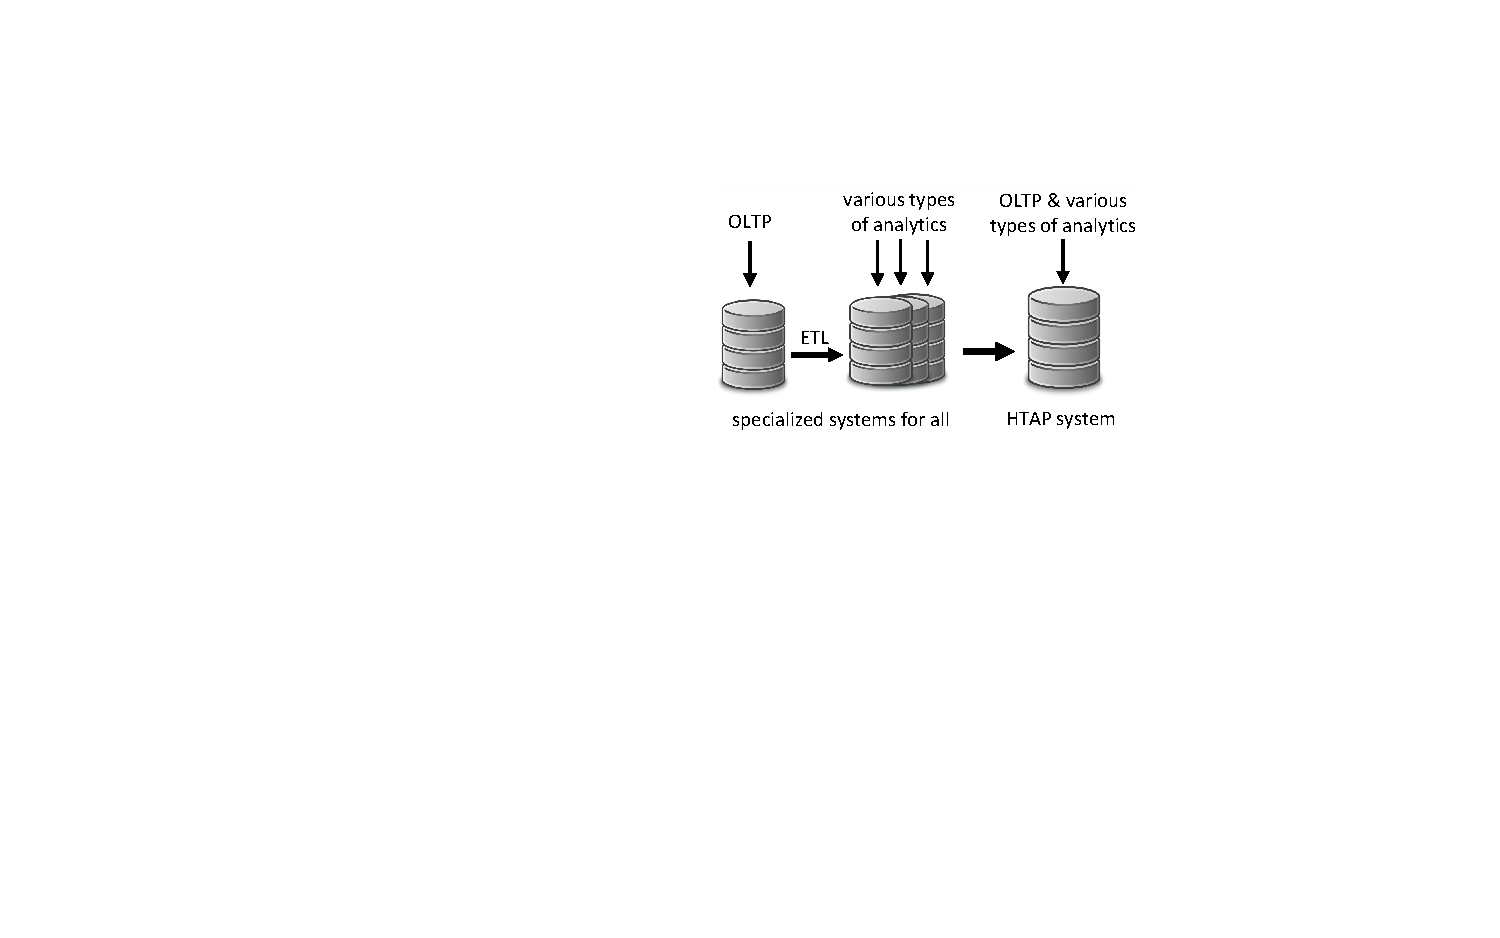
\includegraphics[width=0.4\textwidth]{fig-dia.pdf}}
\caption{(a) Evolution of server hardware over time following Moore’s Law and Dennard Scaling.
Each break in the timeline represents a disruptive period for processor evolution due to power concerns.
(b) Ways to deploy data-intensive applications.}
\label{fig:hwdia}
\end{figure}

% the server hardware gives us different types of parallelism ... in one paragraph and picture maybe
Server hardware has gone through major advances over the years as illustrated in \reffig{hw}.
These advances have stemmed from Moore’s Law \cite{Moore65},
which is the observation that the number of transistors in a dense integrated circuit doubles approximately every two years.
To exploit the increase in the transistor counts in a unit area, initially,
computer architects focused on boosting the performance of a single core while designing chips
(left-hand side of \reffig{hw}).
Around 2005, however, Dennard Scaling \cite{DennardGYRBAL74},
which states that as the transistors get smaller their power density in a unit area remains constant, came to a halt.
Increasing the complexity of a processor core became non-viable since it raised concerns about power draw and heat dissipation.
To overcome this limitation, computer architects started to add more and more cores on a single processor \cite{OlukotunNHWC96}
and more and more processors in servers (middle part of \reffig{hw}).
Multicore processors have enabled the continuation of Moore’s Law despite the halt of Dennard Scaling.
Unfortunately, the limits of the traditional multicore processor design is also upon us. 
Adding more and more cores to a processor cannot be the only path to overcome the halt of Dennard Scaling
since we will not be able to power all of those cores up simultaneously.
This trend is also known as dark silicon \cite{EsmaeilzadehBASB11}.
To overcome this limitation, we must design cores that are more energy-efficient.
One way to achieve this by specializing cores, reducing energy spent per instruction, for certain tasks \cite{HennessyP19}.
Then, as part of the commodity servers, one can utilize the specialized cores in addition to the general-purpose ones.
%which forces us to commoditize alternatives to general-purpose processors
%to optimize energy spent per instruction \cite{HennessyP19}.
The emerging server hardware landscape, therefore,
will likely to be composed of a heterogeneous set of processing units
(as illustrated by the different colors in right-hand side of \reffig{hw});
each specialized to execute a specific task very well,
with opportunities for extreme levels of parallelism.

% variety of applications 
In parallel to the evolution of commodity server hardware that data-intensive applications typically run on,
the applications themselves and how they are deployed have also changed over time as illustrated in \reffig{dia}. 
Transaction and analytical processing used to be the two broad categories of data-intensive applications.
Analytics, in turn, have several distinct sub-categories such as
online analytical processing, data warehousing, machine learning, graph analytics, etc.
Traditionally, they have been deployed separately and data moved from an operational system
(such as an online transaction processing system)
to various types of analytics systems using an extract-transform-load (ETL) process. 
The reason for this separation is that optimal system design for serving
transactional and different types of analytical tasks are different
(e.g., row stores for OLTP, column stores for OLAP, NoSQL for unstructured data, etc.).
In recent years, however, the popularity of the data-intensive applications such as 
real-time inventory/pricing/recommendations, fraud detection, risk analysis, IoT, AI, etc.
require data management systems that can run fast transactions and analytics simultaneously.
As a result, there is an increasing demand for data management systems that can handle
hybrid transactional and analytical processing (HTAP) efficiently \cite{OzcanTT17}.

% the purpose of this text is to survey scheduling methods and challenges in three parts of this picture 
Designing a scheduling mechanism that is able to leverage the heterogeneity of
processing units for the variety of the data-intensive tasks to be executed
in the emerging hardware and software landscapes is a difficult but significant challenge to tackle. 
The goal of this article is to derive some guidelines to overcome this challenge
in the context of a single node of commodity server hardware.
First, \refsec{sched}
surveys some of the existing work that target scheduling of data-intensive tasks on modern homogeneous multicore servers.
Then, \refsec{het} discusses emerging heterogeneous server hardware landscape and
considers existing work in the context of such hardware.
Finally, \refsec{guide}
illustrates a framework for scheduling diverse set of (or hybrid) data-intensive tasks
over diverse set of (or heterogeneous) processing units focusing on the resource estimation challenges.

\section{Scheduling Data-Intensive Tasks over Different Dimensions of Parallelism}
\label{sec:sched}

As previously mentioned,
we view the effective scheduling of different data-intensive tasks as a significant factor
when it comes to effective utilization of the resources of modern server hardware.
Any mechanism that targets effective scheduling must be able to answer the following questions. 

\textit{\textbf{What} to schedule?}
This question determines the unit of scheduling.
What is the granularity of the task to be executed on a specific processing unit?
Is it the whole data-intensive task required by a client request or is it part of it?
If it is a part of it, what is the size of that part?

\textit{\textbf{Where} to schedule?}
This challenge handles the mapping between tasks and processing units.
This mapping has both a \textit{static} and a \textit{dynamic} part.
The static mapping targets the question of what the most effective processing unit/units to execute a task is/are.
The answer to this question assumes that every kind of processing unit is available in infinite amounts.
In practice, however, we rarely have all kinds of processing units in a single server and the hardware resources are finite.
The dynamic mapping must consider the question of whether the ideal processing units
for a task are available at the exact time that we have to execute that task.
In addition, in the case of unavailability, what are the next best alternatives?

\textit{\textbf{How} to schedule?}
This challenge provides the necessary execution and communication primitives,
especially if multiple processing units are involved in executing a task.
What are the primitives to utilize while scheduling a task or parts of a task?
Which level(s) of the system stack these primitives come from? 

The following subsections survey the scheduling mechanisms proposed in recent work that
depart from the conventional wisdom when it comes to the answers to the questions above.
\refsec{sched:impl} and \refsec{sched:expl} focus on utilizing the resources of
a single core and multiple uniform cores, respectively.

\subsection{Implicit/Vertical Parallelism}
\label{sec:sched:impl}

Before Dennard Scaling made it problematic to put more complexity within a core due to heat dissipation concerns,
exploiting Moore's Law meant boosting the performance of a single core.
This resulted in parallelism opportunities within a core through techniques like
instruction level parallelism, pipelining, out-of-order execution, simultaneous multithreading, etc.
We refer to this kind of parallelism as \textit{implicit/vertical} parallelism
as the different tasks are time-multiplexed on the same core
instead of being run concurrently in the same execution cycle.
The main insight behind this kind of parallelism is overlapping various stall times with other work
instead of a core wasting the execution cycles being idle.
For example, as a core waits for fetching an instruction or data item from memory due to it not being present in L1 caches,
one can overlap this waiting time with another instruction or data fetch request from the same task
or execute another task on the same core.
In addition, mostly hardware manages this kind of parallelism and software has the luxury to be oblivious to it.
Therefore, before multicores emerged,
the software systems got faster with each new generation of servers without having to make fundamental design changes.

On the other hand, 
for many data-intensive applications being oblivious to implicit parallelism leads to severe underutilization of
the micro-architectural resources of servers.
Several workload characterization studies emphasize the high rates of memory access related stall times
due to either instruction or data accesses for data-intensive applications \cite{Ferdman+12, SirinTPA16}.
Similarly, techniques like simultaneous multithreading may even hurt performance if not used carefully \cite{ZhouCRS05}.
Multiple data-intensive tasks sharing the same resources in a core simultaneously may put more pressure on caches
due to their aggregate data and instruction footprint.
Therefore,
there is value to rethink the way we design and schedule data-intensive tasks even when utilizing implicit parallelism.

\begin{figure}
\centering
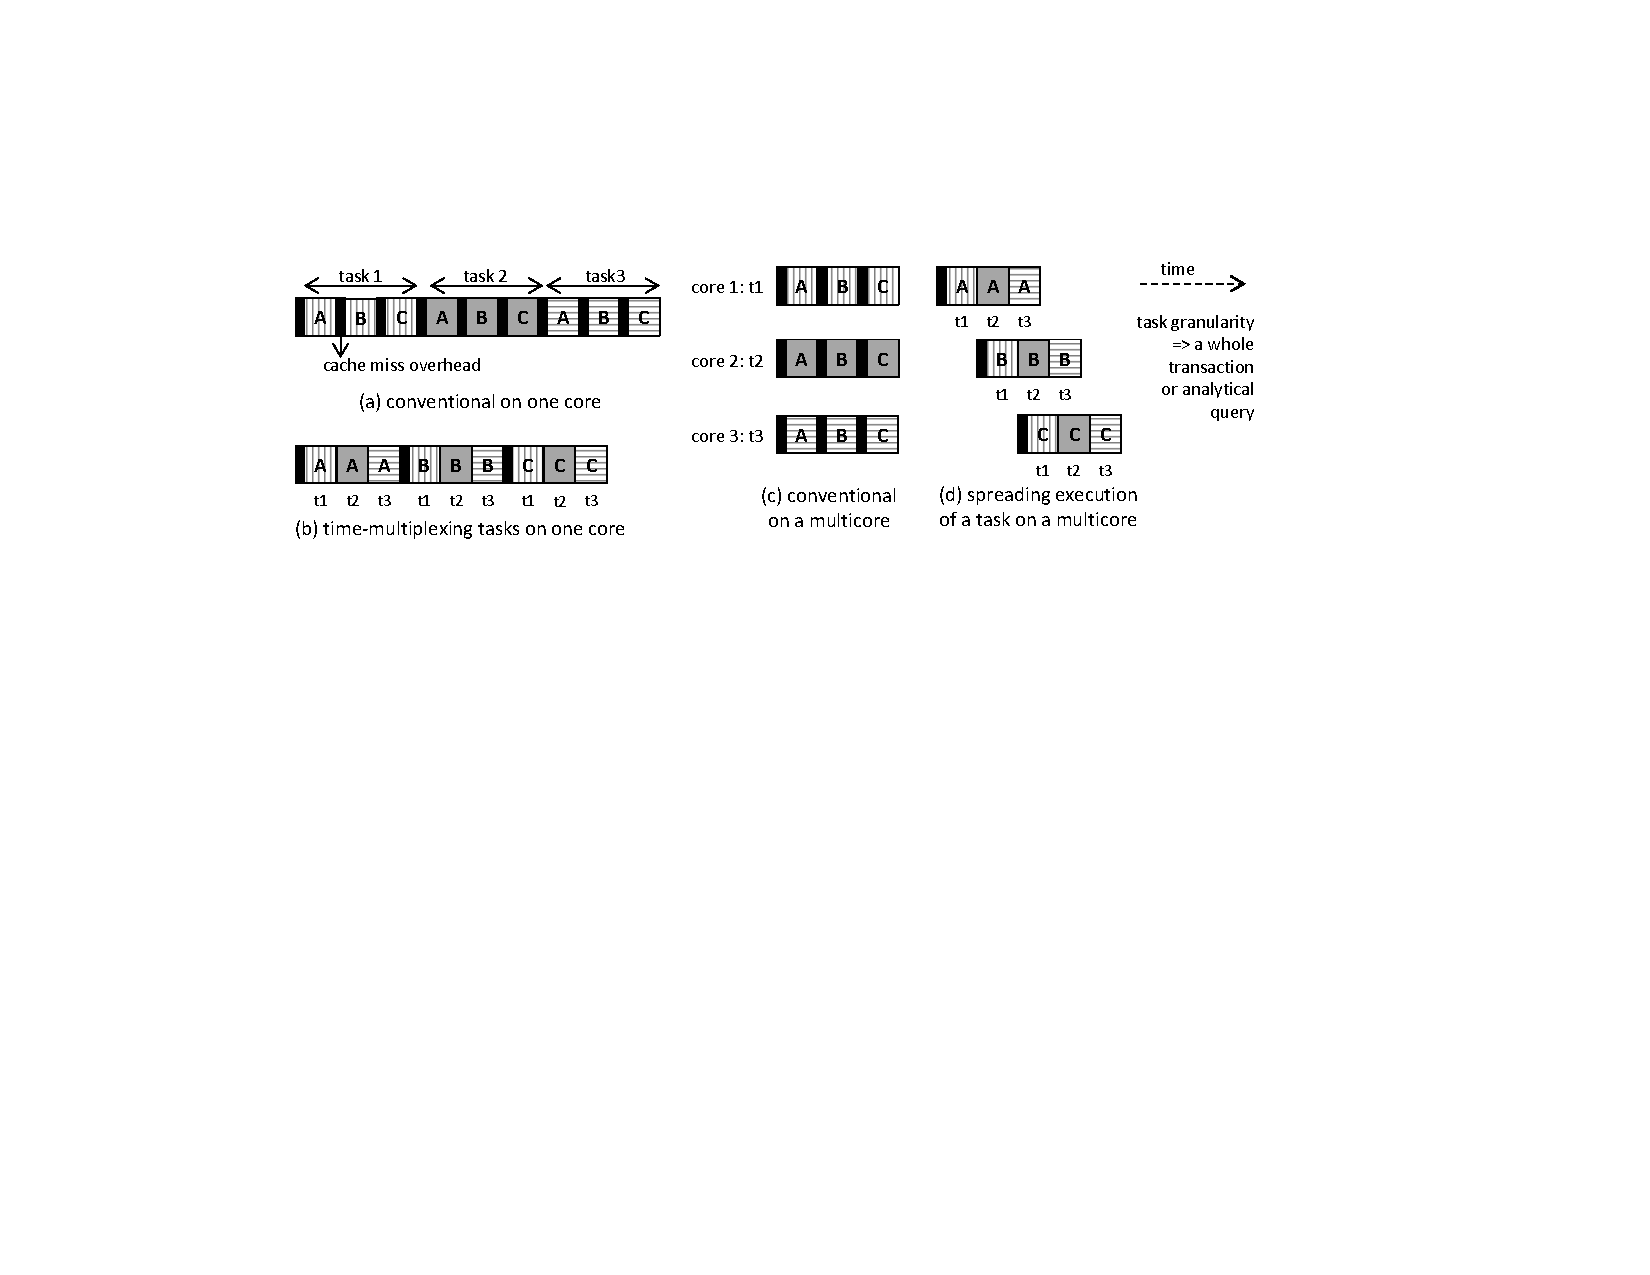
\includegraphics{fig-sched.pdf}
\caption{Different ways of scheduling data-intensive tasks.
%on one core (a \& b) and on a multicore (c \& d) assuming no context switching due to I/O.
In the context of this illustration a task is at the granularity of a transaction or an analytical query,
where A, B, and C are the sub-tasks of this task.}
\label{fig:sched}
\end{figure}

\reffig{sched} illustrates alternative ways of scheduling a data-intensive task
on a single core (a \& b) and on multiple cores (c \& d).
The figure assumes that tasks run over a setup that has fast I/O (e.g., DRAM, NVRAM, low-latency SSD)
and hence do not require context switching due to slow I/O (e.g., HDD).
%assuming the tasks can run without any context switching due to I/O.
In the figure, a data-intensive task is at the granularity of a whole transaction or analytical query.
The task has three sub-tasks A, B, C.
In the interest of our discussion, let's assume that these sub-tasks are at a granularity
where their instruction or data set sizes can fit in L1-I or L1-D, respectively.
This section discusses \reffig{sched}(a \& b) since the focus is on implicit parallelism,
whereas the discussion of \reffig{sched}(c \& d) is in \refsec{sched:expl}.

\reffig{sched}(a) depicts the more conventional way of scheduling tasks.
In this case, the tasks run without any interruptions on a core as a whole one after the other
based on their priority in a task queue in the system.
They take turns thrashing the caches since each executes sub-tasks A through
C in order independent of the other tasks.
Thus, each sub-task incurs overhead due to cache misses.
In this case,
the answer to the \textit{what} question is the whole task
while the \textit{where} question doesn't matter as there is only a single core,
and the answer to the \textit{how} question is mainly left to the default mechanisms
supported by the operating system.

\reffig{sched}(b) shows an alternative way to schedule the sub-tasks,
which time-multiplexes them with the goal of maximizing cache locality.
The first, \textit{lead}, task executes A incurring cache miss overhead as previously.
However, instead of proceeding to execute B, the first task context switches allowing,
in turn, the second and third tasks to execute instead.
The second and third tasks find sub-task A in L1 and thus incur no overhead due to misses.
Once all three tasks execute the first sub-task, execution proceeds to the second one and so on.

The core idea of time-multiplexing the tasks on a single core to improve cache locality
has been studied and shown to be effective in the context of both
instruction (L1-I) and data (L1-D) \cite{AttaTTAM13, HarizopoulosA04, HarizopoulosSA05, LarusP02} locality.
The main insight behind this idea is that similar tasks share common instructions or data or both.
As a result, they can benefit from constructive sharing of the cache resources to improve locality.
Fewer cache misses lead to better utilization of the micro-architectural resources
that enable implicit parallelism within a core
since a smaller portion of the overall execution time is spent on stalls. 
Even if a technique that focuses on instruction cache locality may hinder data cache locality or vice-versa,
the benefits of one may outshine the overhead of the other,
or the locality may improve at the higher levels of the cache hierarchy
despite the hindered L1 locality thanks to constructive sharing \cite{TozunAAM14}.

Achieving constructive sharing for different concurrent tasks in a system is not straightforward.
The first challenge is the underlying assumption of the tasks would have similar sub-tasks to be executed.
For data-intensive applications, this is not an issue.
No matter how different the output or high-level functionality of one data-intensive task from another,
data management or processing systems typically compose a subset of predefined sub-tasks to serve a task.
\reffig{common} and \reffig{intratask}
show some examples within the same or across different applications/tasks.
Transactions are composed of sub-tasks such as probing and scanning an index,
inserting a tuple to a table, updating a tuple, etc.
Traditional analytical queries are composed of projections, selections, joins, etc.
These sub-tasks themselves have common sub-tasks such as hash table lookup, data partitioning, sorting, etc.
across different types of sub-tasks or workloads.
There may be frequently accessed tables or indexes or metadata used by several of these sub-tasks.
Overall, there are many opportunities for constructive sharing in data-intensive applications.

Determining the granularity of sub-tasks to time-multiplex at runtime is a harder challenge
(to answer the \textit{what} question)
as well as orchestrating the runtime scheduling in a lightweight manner
(to answer the \textit{how} question).
Regarding the former challenge,
previous work either considers the granularity of database operators \cite{HarizopoulosSA05},
rely on monitoring the cache behavior at runtime
to determine when the L1 cache starts to become full \cite{AttaTTAM13},
or perform profiling \cite{HarizopoulosA04}.
Regarding the latter challenge,
previous work either adopts hardware mechanisms \cite{AttaTTAM13}
to sidestep the overheads of default context switching primitives of the operating system,
or develop specialized context switching at the kernel-level \cite{HarizopoulosA04}.

Finally, despite increasing the throughput,
time-multiplexing a batch of tasks on one core increases the average latency,
especially for the \textit{lead} task.
One has to take into account the priority or latency requirements of
the data-intensive tasks when deploying these types of scheduling mechanisms.
This challenge is definitely under-studied in the literature.

\begin{figure}
\centering
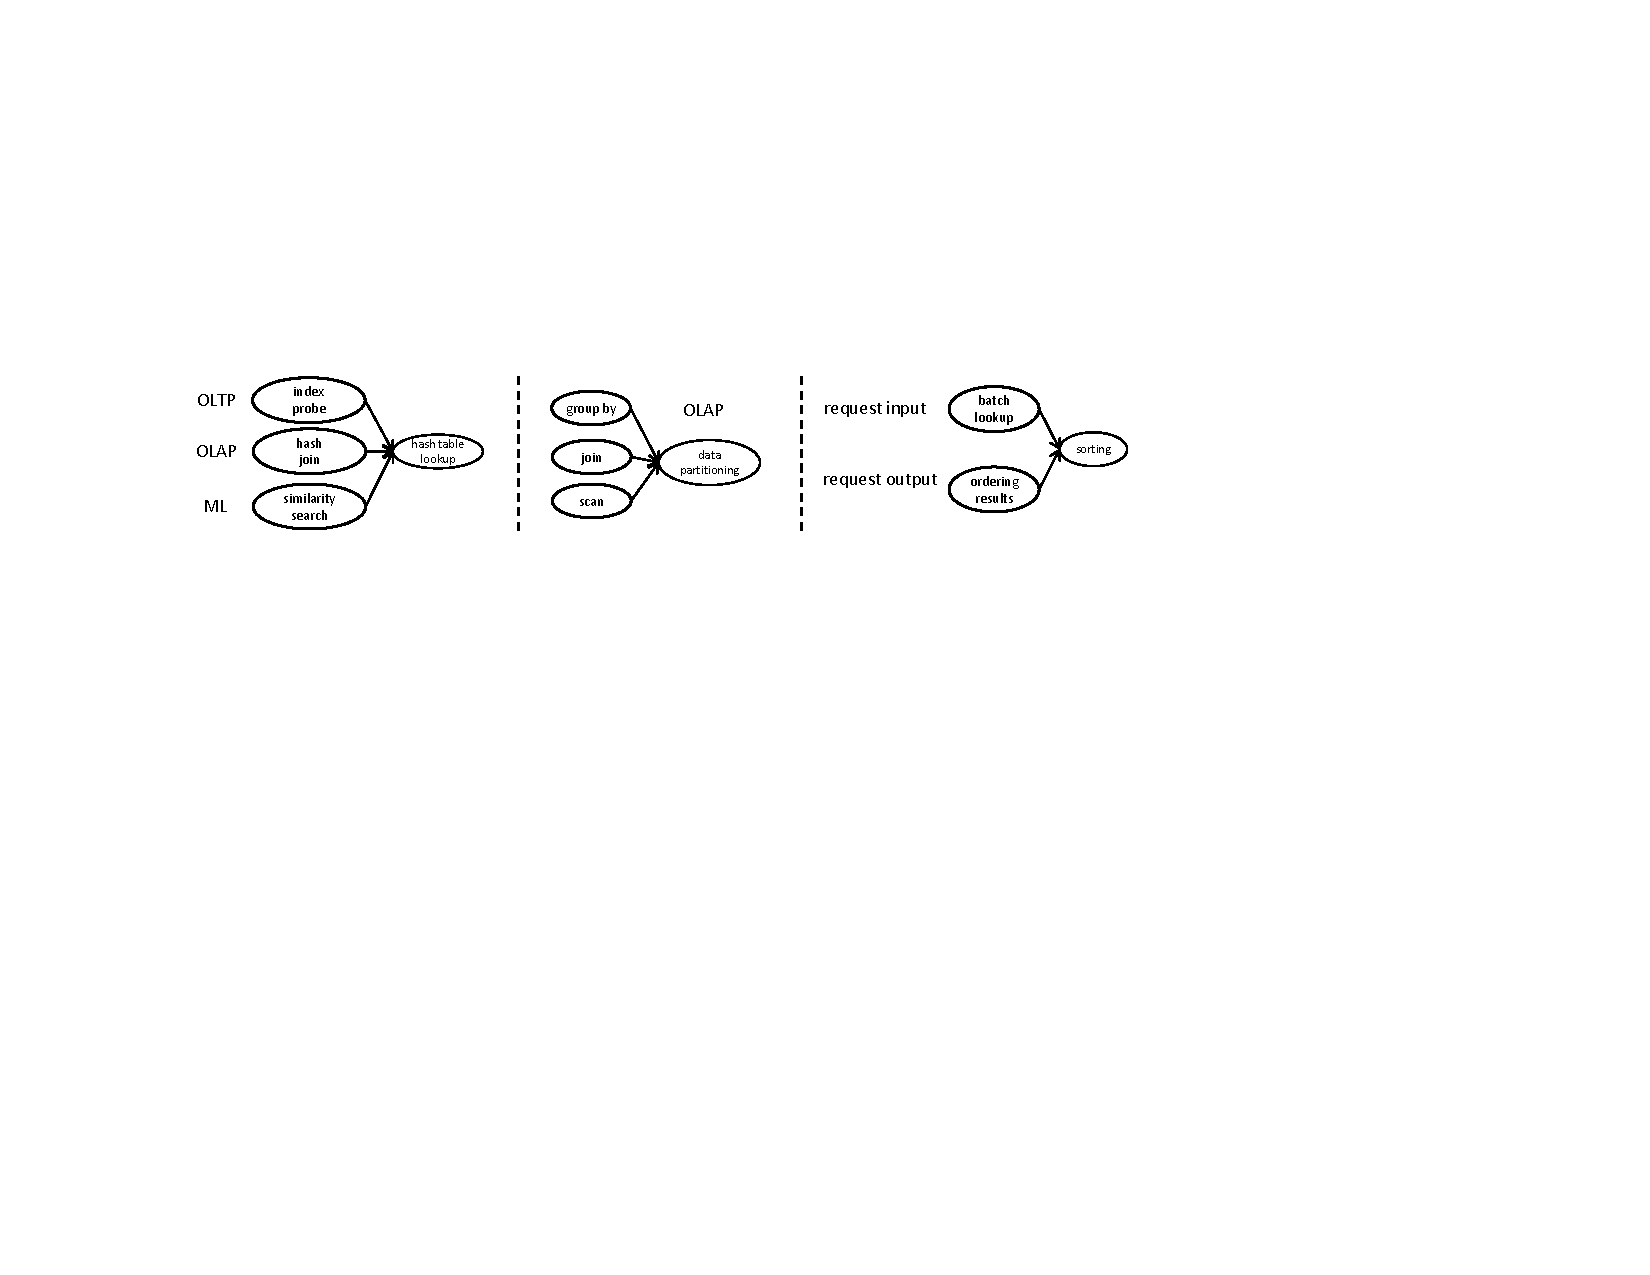
\includegraphics{fig-common.pdf}
\caption{Examples of common sub-tasks across different types of data-intensive applications.
Hash table lookup is common across OLTP, OLAP, and machine learning.
Data partitioning is common across many OLAP tasks.
Sorting is common both across data-intensive applications and
while ordering input/output values from various client requests.}
\label{fig:common}
\end{figure}

\subsection{Explicit/Horizontal Parallelism}
\label{sec:sched:expl}

The switch to multicore processors forced traditional software systems,
including data management systems,
to go through fundamental design changes in order to exploit
the kind of parallelism offered by having multiple cores in a processor \cite{AilamakiLTPP17}.
We refer to this kind of parallelism as \textit{explicit/horizontal} parallelism
as it allows different tasks to run simultaneously in the same execution cycle.
Unlike implicit parallelism,
this type of parallelism has to be managed more carefully at the software side to reap the benefits.
In this dimension of parallelism,
majority of the efforts from previous work focus on removing scalability bottlenecks that arise
due to concurrent threads accessing shared data.
Complementary to such scalability problems,
this article focuses on the work that targets scheduling of data-intensive tasks on multicores.

Let's start by following the discussion from \reffig{sched},
\reffig{sched}(c \& d) illustrate alternative ways of scheduling data-intensive tasks on multicores.
\reffig{sched}(c) depicts the more conventional way when there is no I/O.
Each task is scheduled to a different core in the system and executed as a whole on that core.
As a result, each task exhibits cache misses
since neither the instruction nor the data footprint of data-intensive tasks fit in L1 caches.
This way of scheduling stems from traditional data management systems treating various
data management tasks as large indivisible units of work on a single server.
This monolithic view of such tasks eventually leads to sub-optimal resource management
decisions even on today's homogeneous commodity server hardware \cite{TozunAAM14}.

In the case of \reffig{sched}(c), just like \reffig{sched}(a),
the answer to the \textit{what} question is the whole task
and the answer to the \textit{how} question is mainly left to the default mechanisms supported by the operating system.
On the other hand,
having multiple cores makes the \textit{where} question more difficult to answer.
Traditional systems typically pick the next available/idle core to schedule the next task to be executed.

\reffig{sched}(d), on the other hand, 
spreads the computation of a data-intensive task over multiple cores and
utilizes the aggregate L1-I cache capacity of the multicores while executing this task.
The main insight behind this idea is, as in \refsec{sched:impl}, the observation that
data-intensive tasks in general share common sub-tasks (or code \cite{TozunAAM14}).
As long as there are enough cores so that the aggregate L1-I capacity can hold all code segments,
a task can migrate to the core whose L1-I cache holds the code segment the task is about to execute.
For example, as \reffig{sched}(d) shows,
the first, \emph{lead}, transaction can execute sub-task A first on core 1,
then migrate to core 2 where it would execute sub-task B,
then migrate to core 3 where it would execute sub-task C.
The second and third tasks can follow in a pipelined fashion,
finding sub-tasks A, B, and C, in cores 1, 2, and 3, respectively.
While the lead task incurs an overhead when fetching the code segments for the first time,
the other tasks do not.
Even though, the migrations may diminish data locality at the L1-D level,
as long as they happen within a processor/socket,
long-latency data misses from the last-level cache either stay the same
or get reduced as a result of constructive data sharing across similar tasks \cite{TozunAAM14}.

The core idea of spreading the computation over multiple cores to improve instruction cache locality,
is initially studied in the context of separating kernel code from application code in \cite{ChakrabortyWS06}.
SLICC \cite{AttaTAM12-2} and ADDICT \cite{TozunAAM14} have taken this idea further 
to also localize the common application code across concurrent data-intensive tasks over specific cores.
These work in fact target improving cache locality,
minimizing stall times due to cache misses,
and hence, improving utilization of implicit parallelism within a core
like the work described in \refsec{sched:impl}.
However, they exploit explicit parallelism to achieve their target.
Similarly, the staged execution mechanisms such as QPipe \cite{HarizopoulosSA05},
which are originally developed with implicit parallelism in mind,
are later adapted to utilize explicit parallelism as well \cite{GiannikisAK12, PsaroudakisAA13}.
Furthermore, separating the tasks to be executed by the kernel and the data-intensive application
into common sub-tasks, and running these sub-tasks over separate specific cores is also
studied in the context of effective operating system and database system co-design \cite{GicevaZAR16}.

In addition to strengthening the techniques that
target improving (instruction or data) locality for data-intensive tasks,
explicit parallelism also allows exploiting intra-task parallelism.
In other words, 
the independent sub-tasks of a data-intensive task can run concurrently over multiple cores.
To prevent underutilization of ever increasing explicit parallelism offered by multicores or many cores,
intra-task parallelism is essential.
Viewing tasks as a black-box and just focusing on optimizing for inter-task parallelism
is ineffective while scaling up on servers with 100s or 1000s of cores.

A common way to achieve intra-task parallelism is to partition the data to be processed
by a data-intensive task and assign different threads to each partition \cite{LeisBKN14, PsaroudakisSMSA15}.
Data partitioning is only one dimension when targeting intra-task parallelism, though.
The other, slightly more challenging, dimension is to detect the independent sub-tasks
within a task that can run concurrently. 
\reffig{intratask} gives an example of how to parallelize the sub-tasks of the
\texttt{payment} transaction from the industry-standard TPC-C benchmark \cite{TPCC},
which is utilized by the DORA/PLP mechanisms \cite{Pandis+11, PandisTJA11}.
The three update operations over the different tables (customer, district, and warehouse)
have no dependency on each other and can run in parallel
while the insert operation over the history table must run after these three.
Previous work adapted the SQL frontend of Postgres to determine the independent
sub-tasks of transactions automatically \cite{Pandis+11}.
Expanding this methodology to more complex data-intensive tasks is still a challenge.

All the mechanisms that involve multiple cores in the execution of a transaction
whether it is to improve cache locality or intra-task parallelism or both,
have the same challenges as the mechanisms that time-multiplex sub-tasks on the same core (\reffig{sched}(b)).
Therefore, the answers to the \textit{what} and \textit{how} questions here are the same as in \refsec{sched:impl}
(i.e., finer-granularity sub-tasks and lighter-weight context switching).
Answering the \textit{where} question, on the other hand,
requires runtime monitoring and bookkeeping to know which core has the instructions a sub-task needs
or which cores are assigned to which database operators beforehand.
Furthermore,
explicit parallelism in the era of multisocket multicore hardware with non-uniform memory access (NUMA),
also brings the challenge of minimizing communication overheads across the sub-tasks.
Involving multiple cores in the execution of a data-intensive tasks require orchestrating the sub-tasks,
which requires communication across cores that may not be able to communicate as fast as some other cores.
Naive ways of scheduling sub-tasks ignoring hardware topology, especially NUMA,
may hinder overall performance even if it utilizes explicit parallelism well \cite{PorobicLTA14, PsaroudakisSMSA15}.
Therefore, one must definitely take the hardware topology into account while answering the \textit{where} question.

\begin{figure}
\centering
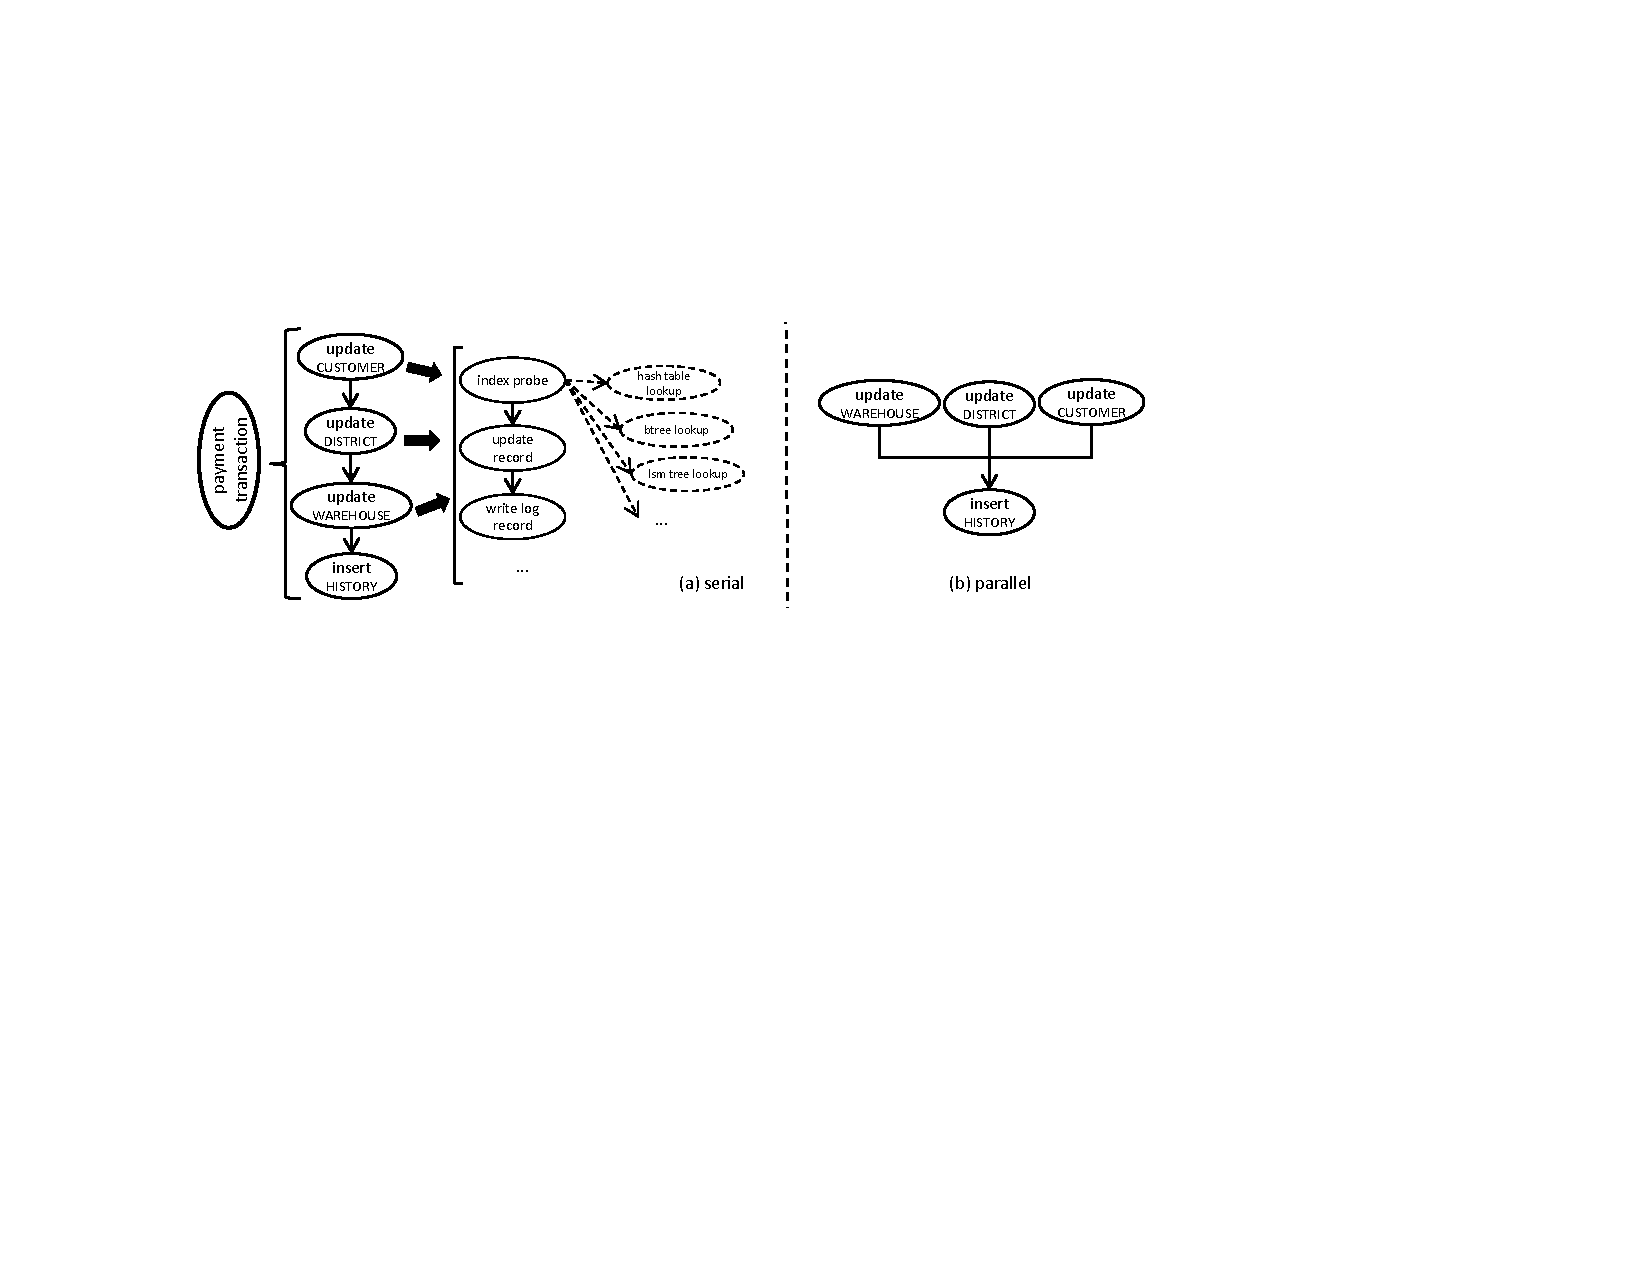
\includegraphics{fig-intrataskgran.pdf}
\caption{TPC-C's \texttt{payment} transaction.
Each node represents a sub-task in \texttt{payment}.
\texttt{Customer}, \texttt{District}, \texttt{Warehouse}, and \texttt{History} are the tables in TPC-C.
(For brevity the iteration over the \texttt{Customer} table in this transaction is omitted).
(a) The serial execution plan also illustrating the sub-tasks of \texttt{payment} at different granularities.
\texttt{payment} performs operations such as update and insert.
An update performs actions such as index probe, update record, write log, etc.
These actions also have sub-tasks at a finer-granularity.
(b) The parallel execution plan for \texttt{payment}
exploiting intra-transaction parallelism among the three independent updates.}
\label{fig:intratask}
\end{figure}

\section{Toward Heterogeneous Parallelism}
\label{sec:het}

As mentioned in \refsec{intro},
adding more and more cores to a processor cannot be the only path for progressing commodity servers anymore.
Moore's Law is slowing down.
The main reason is once again power-related even though there are other physical constraints as well
(e.g., fabrication costs for transistors that get smaller and smaller).
The supply voltage required to power all the transistors up does not decrease at a proportional rate.
Even if we can still add more and more cores on processors,
we will not be able to power all of them up simultaneously \cite{EsmaeilzadehBASB11}.
Optimizing energy per instruction has to be the key in this new era.

One option to achieve more energy-efficient hardware is to adopt simpler and more low-power cores in emerging processors.
However, such processing units are not suitable for latency critical applications.
In addition, solely focusing on the energy-efficiency of an individual core or processor
is not going to give us energy-proportionality \cite{BarrosoH07}.
We have to focus on how much energy it takes to run tasks to completion.
The low-power cores might end up spending more energy at the end of the day for running a set of tasks 
compared to power-hungry cores since it takes them longer to execute tasks due to being slower \cite{LangPS10}.

The better long-term solution for energy-efficiency is to build servers with a variety of processing units,
where each unit is specialized to accelerate specific tasks.
On such servers, one would pick the cores to power-up based on the tasks currently running,
while shutting down the idle cores that are specialized for other types of tasks.
Orchestrating task scheduling dynamically over such heterogeneous hardware intensifies
an already challenging problem on homogeneous hardware (as \refsec{sched} focused on).
In addition, economic feasibility of specialized hardware is always a concern
since specialization limits the market of a system, despite being more efficient,
as opposed to being general-purpose.
%
As a result, processor specialization for data-intensive tasks was unpopular in industry up until recently.
However, this attitude has been changing \cite{AlonsoB18, HennessyP19}. %\cite{catapult, tpu}.
%First, the growing size of data and complexity of data-intensive applications require more and more processing power.
%The slowdown of the evolution of today’s commodity multicore servers require departing from conventional thinking. 
%Second, the increasing scale of the data-intensive applications has started to diminish the economic concerns over specialized hardware.
%Third, the tools that enable more uniform programming interfaces over heterogeneous hardware have been maturing.
%Fourth, major server hardware vendors have been designing products with different types of processing units targeting data-intensive applications.
Therefore, there is pressing need to develop scheduling mechanisms that not only consider
the diversity of the data-intensive tasks, but also the diversity of the processing units.

The scheduling approaches surveyed in \refsec{sched} are inspiring and preliminary steps
toward the efficient utilization of processors with many diverse parallelism opportunities.
The common denominators (and the common root of the associated challenges)
across all of these mechanisms are that
(1) they view data-intensive tasks at a finer sub-task granularity
(e.g., \textit{update} operation of \textit{payment} transaction instead of the whole \textit{payment} transaction)
and (2) they adopt lighter-weight and hardware-topology-aware techniques for dynamic scheduling of these sub-tasks
instead of relying on the traditional operating system defaults.

Splitting data-intensive tasks into their sub-tasks
(see examples in \reffig{common} and \reffig{intratask})
help in identifying the common sub-tasks across concurrent transactions or analytical queries.
This, in turn, enables more opportunities for constructive instruction and data sharing,
intra-task parallelism, and mapping a unit work to a core that would benefit the most from running on that core.
Furthermore, it is an essential preliminary step to 
discover the frequent critical sub-tasks that justify building new specialized hardware for.
Therefore,
even though detecting the right granularity for sub-tasks and orchestrating more things at runtime is a big challenge,
this challenge is worthwhile to address and study in more depth.
It is the only way to answer the \textit{what} question and aides answering the \textit{where} question
in the context of emerging heterogeneous hardware landscape.

After mapping a certain granularity of sub-tasks to the available processing units at runtime,
one has to perform the actual scheduling and coordination of these sub-tasks efficiently.
Otherwise, no matter how optimal the mapping is, it is not going to be beneficial.
Specializing context switching or thread migrations for data-intensive tasks
either at the level of the kernel or hardware has been tried (as also mentioned in \refsec{sched:impl}).
These techniques and others that specialize the same routines
should be revisited in more detail in the context of heterogeneous hardware.
It is highly likely that the common operating system layers and mechanisms will also evolve with such hardware.
Therefore, it is important to have a holistic view while developing mechanisms to efficiently coordinate sub-tasks
in order to achieve lightweight coordination and minimize replication of functionality across layers.
In addition, exploiting more and more processing units should not turn the development
of a data-intensive application into an unproductive process.
Ensuring the correct and efficient instruction and data stream on a specific processing unit should be handled through
high-level language primitives for the application developer and smart query compilation within the data management system
\cite{HeimelSPMM13}.
%\cite{HeimelSPMM13, PirkMZM16}.
Tackling these two challenges is the way to answer the \textit{how} question for heterogeneous many cores.

Next, we discuss an end-to-end framework that takes the challenges of scheduling varying data-intensive tasks
on heterogeneous hardware into account by mainly focusing on the resource estimation challenge,
which also aides the \textit{where} question.

\section{A Framework for Running Data-Intensive Tasks on Emerging Hardware}
\label{sec:guide}

Even though the previous sections focus on the utilization of a single server hardware,
resource-aware scheduling is an active field of research often tailored specifically for different hardware platforms,
from small embedded systems~\cite{Tillenius_2015} up to clusters~\cite{Delimitrou_2014}.
Executing tasks with varying resource demands in parallel can lead to inefficient resource utilization,
especially on heterogeneous hardware.
More precisely, the correlation between the resource demand of a task and its completion time is often highly non-linear,
once the task is executed concurrently with other ones.
In order to solve the very challenging problem of finding an optimal resource mapping for a single task,
new resource-aware scheduling strategies are required,
which efficiently map tasks to heterogeneous parallel architectures,
taking their particular resource demands into account. 
Independent of the actual objective,
i.e., making the execution of hybrid tasks more efficient or
designing an efficient parallelization strategy for a specific task,
the underlying motivation remains the same, namely,
optimizing the execution of tasks on heterogeneous hardware architectures while respecting given latency requirements.

In data management systems,
hybrid data-intensive tasks often arrive dynamically
providing only inaccurate information about their resource utilization behavior.
Unlike classical scheduling problems, such systems require mapping methods that
(1) interact with a resource model to map tasks to suitable resources at runtime and
(2) adjust mapping decisions dynamically depending on the system load. 

Many existing work that tackle the problem of scheduling tasks on parallel architectures
aim to optimize either the execution of tasks having similar characteristics (e.g., only transactional workloads) or
the scheduling of tasks with hybrid characteristics (transactional and analytical workloads) on homogeneous parallel systems.
For example, database systems such as SAP HANA or HyPer are designed to efficiently execute hybrid tasks
using an optimized workload management system for servers with homogeneous cores~\cite{Psaroudakis_2015}.
Future scheduling strategies, however, should consider both the heterogeneity of workloads and of hardware
in order to find an efficient resource-aware mapping exploiting the full potential of the underlying parallel architecture.

To enable a resource-efficient scheduling of data-intensive tasks over complex heterogeneous hardware architectures,
we focus on a framework, illustrated in \reffig{framework},
that includes scheduling mechanisms guided by resource estimation models.
Regarding different aspects of our strategy,
we survey previous approaches harvesting already existing results that shall serve as a guideline.

To generate resource estimation models distinct machine learning methods or analytical models
can be applied to predict the resource demands for different possible task-to-core(s) mapping strategies.
Analytical models can be more accurate than machine learning models
when applied to estimate the runtime of concurrently executed tasks~\cite{Wu_2013}.
However,
machine learning models are typically preferred in more complex heterogeneous hardware scenarios,
since the complexity of the analytical models can increase rapidly in such cases. 
When building models that are capable of describing the complete data management system behavior,
several aspects need to be taken into consideration.
For models with high multidimensionality and thus high complexity,
a dimensionality reduction, through machine learning techniques such as clustering or classification,
is suggested~\cite{Chen_2011}.
For example, as shown by previous work \cite{Ma_2018},
a workload forecasting strategy based on machine learning techniques can try to predict
the expected arrival rate of certain types of tasks in a data management system
and use clustering to reduce the model complexity.
In general, machine learning methods, especially for resource estimations,
are not only applicable to data management systems running on a single server.
They can also be applied in the context of cluster management,
e.g., to classify heterogeneous workloads that would achieve an efficient resource utilization~\cite{Delimitrou_2014}.

\begin{figure}
	\centering
	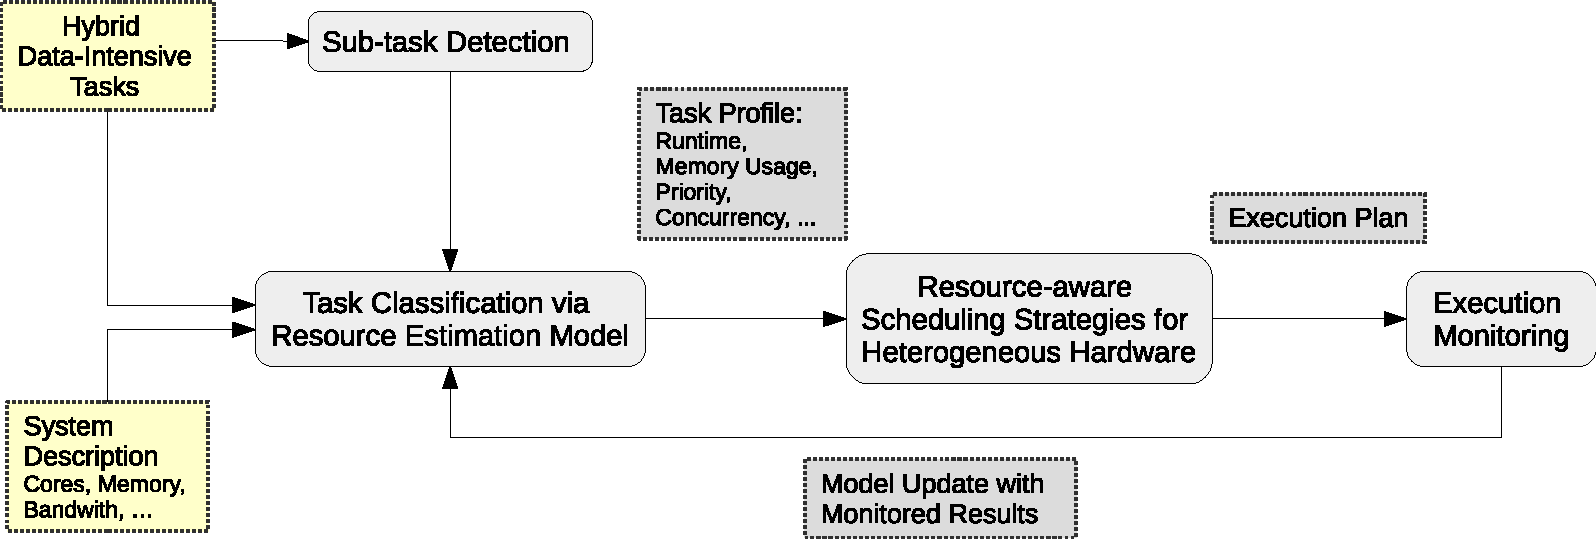
\includegraphics[width=0.95\textwidth]{fig-framework.pdf}
	\caption{Framework for resource-aware scheduling strategies guided by a resource estimation model for hybrid data-intensive tasks executed on heterogeneous hardware.}
	\label{fig:framework}
\end{figure}

\reffig{framework} visualizes the optimization cycle of the resource-aware scheduling framework.
It consists of four main steps.

In the \textit{first} step,
the sub-task detection tries to identify possible sub-tasks from the incoming data-intensive tasks
(transactional and different types of analytical) to take possible parallelization strategies into account.

To determine an efficient mapping of tasks to available hardware,
it is necessary to be aware of each task’s (estimated) resource demand.
To this effect, a flexible resource estimation model is constructed in the \textit{second} step,
which estimates the resource demands of each task and sub-task based on previously executed similar tasks.
Since the available hardware architecture influences the runtime behavior of a task,
the model also uses the hardware description as input,
and later should also be able to adapt to hardware changes.
As mentioned above,
such a model can utilize machine learning techniques instead of analytical cost models,
since the analytical models could become very complex
when they have to cope with many different heterogeneous hardware parts in one system.
Depending on the model's estimations,
tasks can be classified into different types of groups based on their resource demands
to later efficiently map them to suitable hardware resources or queues that are assigned to each group.
Therefore, as an output the model produces task profiles
including different resource utilization characteristics and
an execution priority that can be used for latency critical tasks. 
A similar framework for resource-aware scheduling that focuses on scheduling
parallel parameter optimization of machine learning algorithms with heterogeneous tasks
have been studied in \cite{kotthaus_2017a}.
This framework uses a regression model to estimate the runtime of tasks
and computes an execution priority for each task.
This priority is then used as input to schedule these tasks
in a way that minimizes CPU idling on homogeneous clusters.
Further work on this framework showed that its runtime estimation mechanism also works for heterogeneous hardware.
However, for heterogeneous hardware the random forest regression model is found to be more effective since
task execution times form a discontinuous model
because of the additional categorical variable that represents the processor type~\cite{kotthaus_2018}. 
Besides runtime estimation,
the estimation of multiple performance metrics via machine learning techniques
for specific query plans on homogeneous hardware is proposed in~\cite{Ganapathi_2009}.
In~\cite{Mozafari_2013} a detailed overview of different machine learning techniques applicable for estimating multiple metrics for highly concurrent OLTP workloads on homogeneous systems is given, which could be interesting as well for resource estimations on heterogeneous systems. 

As depicted in \reffig{framework},
the obtained task profiles including multiple metrics serve as inputs for the resource-aware scheduling strategies
in the \textit{third} step.
Resulting from this, an execution plan is created that efficiently maps tasks to suitable hardware resources.
While creating the execution plan, this step also determines whether to use intra-task parallelism or
the degree of parallelism for a task based on the available hardware resources and topology.
As mentioned in \refsec{sched:expl}, due to sub-task coordination efforts and non-uniform core-to-core communication costs,
parallel execution plan of a task may not always result in faster execution compared to running a task serially.

Since the profiles are only estimated, under- or overestimation (e.g., of execution times) may occur.
In such cases, a task may need to be rescheduled or stopped to guarantee latency requirements.
This service is performed by the execution monitoring provided by the \textit{last} step of our strategy.
Here, an adaptive operator replacement technique using machine learning for runtime estimation,
as presented in~\cite{Bress_2014},
could be applied, where operator mappings are dynamically adjusted on heterogeneous co-processors.
Moreover, execution monitoring is also used to gather information about the system behavior, such as CPU or memory utilization, and to measure the de facto resource utilization of tasks at runtime. After a task or a group of tasks has finished their execution, the results are collected to iteratively refine the resource estimation model. Evidently, the quality of the scheduling strategy depends on the accuracy of the resource estimation. Hence, the model update entails more reliable estimations over time for the future predictions of the new incoming tasks.

\section{Conclusion}
\label{sec:conc}

In this article,
we focused on scheduling data-intensive applications with different types of tasks
over the processing units of emerging heterogeneous server hardware.
%targeting the resource utilization of such hardware.
Existing scheduling proposals that diverge from conventional methods when utilizing the resources
of a single server with homogeneous multicores already give us essential insights.
Therefore, their challenges should be revisited in the context of emerging heterogeneous hardware.
More specifically, moving forward we should focus on the following:
(1) identifying sub-tasks of data-intensive tasks across different applications,
especially the common ones that allow constructive sharing of instructions and data,
(2) efficient orchestration of these sub-tasks at runtime,
(3) dynamic models to guide us during task-to-core(s) mapping decisions, and
(4) a holistic approach across hardware, operating systems, and data management/processing systems
to keep the systems' layers lightweight.
This article navigated these items giving a high-level overview.
Our goal is to tackle them in more detail in the future.

%% OLD
%We surveyed existing scheduling proposals that diverge from conventional methods
%when utilizing the resources of a single server with homogeneous multicores and different dimensions of parallelism.
%We identified and followed the three critical questions that any scheduling mechanism must answer
%as we discussed the proposals.
%We consider the insights from these proposals to be essential when targeting heterogeneous platforms as well.
%Therefore, their challenges should be revisited in the context of emerging hardware.
%Furthermore,
%we discussed a resource-aware scheduling framework for hybrid data-intensive tasks running on a heterogeneous server
%emphasizing the importance of resource estimation models in such frameworks.
%Even though we mainly focus on the resource utilization of a single commodity server platform
%while running data-intensive tasks in this article,
%there are common challenges across more resource-constrained environments or large-scale clusters
%as well as other complex applications.

\section*{Acknowledgments}
This work was partly supported by Deutsche Forschungsgemeinschaft (DFG) 
within the Collaborative Research Center SFB 876, projects C5 and A3.
The authors would like to thank Jens Teubner, Philippe Bonnet, and Danica Porobic for providing valuable feedback.

%% 
\begin{thebibliography}{10}
\begin{small}
\itemsep=1pt
%\bibliographystyle{abbrv}
%\bibliography{PTdebullMarch}
\bibitem{AilamakiLTPP17}
A.~Ailamaki, E.~Liarou, P.~T\"oz\"un, D.~Porobic, and I.~Psaroudakis.
\newblock {\em {Databases on Modern Hardware: How to Stop Underutilization and
  Love Multicores}}.
\newblock Morgan {\&} Claypool Publishers, 2017.

\bibitem{AlonsoB18}
G.~Alonso and P.~Bailis.
\newblock {Research for practice: FPGAs in datacenters}.
\newblock {\em {CACM}}, 61(9):48--49, 2018.

\bibitem{AttaTAM12-2}
I.~Atta, P.~T\"oz\"un, A.~Ailamaki, and A.~Moshovos.
\newblock {SLICC}: {S}elf-{A}ssembly of {I}nstruction {C}ache {C}ollectives for
  {OLTP} {W}orkloads.
\newblock In {\em MICRO}, pages 188--198, 2012.

\bibitem{AttaTTAM13}
I.~Atta, P.~T\"oz\"un, X.~Tong, A.~Ailamaki, and A.~Moshovos.
\newblock {STREX}: {B}oosting {I}nstruction {C}ache {R}euse in {OLTP}
  {W}orkloads through {S}tratified {T}ransaction {E}xecution.
\newblock In {\em ISCA}, pages 273--284, 2013.

\bibitem{BarrosoH07}
L.~A. Barroso and U.~H\"{o}lzle.
\newblock {The Case for Energy-Proportional Computing}.
\newblock {\em Computer}, 40:33--37, 2007.

\bibitem{Bress_2014}
S.~Bre\ss, B.~K\"{o}cher, M.~Heimel, V.~Markl, M.~Saecker, and G.~Saake.
\newblock {Ocelot/HyPE: Optimized Data Processing on Heterogeneous Hardware}.
\newblock {\em PVLDB}, 7(13):1609--1612, 2014.

\bibitem{ChakrabortyWS06}
K.~Chakraborty, P.~M. Wells, and G.~S. Sohi.
\newblock Computation {S}preading: {E}mploying {H}ardware {M}igration to
  {S}pecialize {CMP} {C}ores {O}n-the-{F}ly.
\newblock In {\em ASPLOS}, pages 283--292, 2006.

\bibitem{Chen_2011}
Y.~Chen, A.~Ganapathi, and R.~Katz.
\newblock {Challenges and Opportunities for Managing Data Systems Using
  Statistical Models}.
\newblock In {\em IEEE DeBull}, volume~34, pages 53--60, 2011.

\bibitem{Delimitrou_2014}
C.~Delimitrou and C.~Kozyrakis.
\newblock {Quasar: Resource-efficient and QoS-aware Cluster Management}.
\newblock In {\em ASPLOS}, pages 127--144, 2014.

\bibitem{DennardGYRBAL74}
R.~H. Dennard, F.~H. Gaensslen, H.-N. Yu, V.~L. Rideout, E.~Bassous, Andre, and
  R.~Leblanc.
\newblock Design of {I}on-{I}mplanted {MOSFET}s with {V}ery {S}mall {P}hysical
  {D}imensions.
\newblock {\em IEEE J. Solid-State Circuits}, pages 256--268, 1974.

\bibitem{EsmaeilzadehBASB11}
H.~Esmaeilzadeh, E.~Blem, R.~St.~Amant, K.~Sankaralingam, and D.~Burger.
\newblock Dark {S}ilicon and the {E}nd of {M}ulticore {S}caling.
\newblock In {\em ISCA}, pages 365--376, 2011.

\bibitem{Ferdman+12}
M.~Ferdman, A.~Adileh, O.~Kocberber, S.~Volos, M.~Alisafaee, D.~Jevdjic,
  C.~Kaynak, A.~D. Popescu, A.~Ailamaki, and B.~Falsafi.
\newblock Clearing the {C}louds: {A} {S}tudy of {E}merging {S}cale-out
  {W}orkloads on {M}odern {H}ardware.
\newblock In {\em ASPLOS}, pages 37--48, 2012.

\bibitem{Ganapathi_2009}
A.~{Ganapathi}, H.~{Kuno}, U.~{Dayal}, J.~L. {Wiener}, A.~{Fox}, M.~{Jordan},
  and D.~{Patterson}.
\newblock {Predicting Multiple Metrics for Queries: Better Decisions Enabled by
  Machine Learning}.
\newblock In {\em ICDE}, pages 592--603, 2009.

\bibitem{GiannikisAK12}
G.~Giannikis, G.~Alonso, and D.~Kossmann.
\newblock {SharedDB: Killing One Thousand Queries With One Stone}.
\newblock {\em {PVLDB}}, 5(6):526--537, 2012.

\bibitem{GicevaZAR16}
J.~Giceva, G.~Zellweger, G.~Alonso, and T.~Roscoe.
\newblock {Customized OS support for data-processing}.
\newblock In {\em DaMoN}, pages 2:1--2:6, 2016.

\bibitem{Hamilton10}
J.~Hamilton.
\newblock {Perspectives - Overall Data Center Costs}.
\newblock
  \url{https://perspectives.mvdirona.com/2010/09/overall-data-center-costs/}.

\bibitem{HarizopoulosA04}
S.~Harizopoulos and A.~Ailamaki.
\newblock {STEPS} {T}owards {C}ache-{R}esident {T}ransaction {P}rocessing.
\newblock In {\em VLDB}, pages 660--671, 2004.

\bibitem{HarizopoulosSA05}
S.~Harizopoulos, V.~Shkapenyuk, and A.~Ailamaki.
\newblock {QP}ipe: {A} {S}imultaneously {P}ipelined {R}elational {Q}uery
  {E}ngine.
\newblock In {\em SIGMOD}, pages 383--394, 2005.

\bibitem{HeimelSPMM13}
M.~Heimel, M.~Saecker, H.~Pirk, S.~Manegold, and V.~Markl.
\newblock {Hardware-Oblivious Parallelism for In-Memory Column-Stores}.
\newblock {\em {PVLDB}}, 6(9):709--720, 2013.

\bibitem{HennessyP19}
J.~L. Hennessy and D.~A. Patterson.
\newblock {A new golden age for computer architecture}.
\newblock {\em {CACM}}, 62(2):48--60, 2019.

\bibitem{kotthaus_2018}
H.~Kotthaus.
\newblock {\em {Methods for Efficient Resource Utilization in Statistical
  Machine Learning Algorithms}}.
\newblock PhD thesis, TU Dortmund University, 2018.

\bibitem{kotthaus_2017a}
H.~Kotthaus, J.~Richter, A.~Lang, J.~Thomas, B.~Bischl, P.~Marwedel,
  J.~Rahnenführer, and M.~Lang.
\newblock {RAMBO: Resource-Aware Model-Based Optimization with Scheduling for
  Heterogeneous Runtimes and a Comparison with Asynchronous Model-Based
  Optimization}.
\newblock In {\em LION}, pages 180--195, 2017.

\bibitem{LangPS10}
W.~Lang, J.~M. Patel, and S.~Shankar.
\newblock Wimpy {N}ode {C}lusters: {W}hat {A}bout {N}on-{W}impy {W}orkloads?
\newblock In {\em DaMoN}, pages 47--55, 2010.

\bibitem{LarusP02}
J.~R. Larus and M.~Parkes.
\newblock {Using Cohort-Scheduling to Enhance Server Performance}.
\newblock In {\em USENIX}, pages 103--114, 2002.

\bibitem{LeisBKN14}
V.~Leis, P.~A. Boncz, A.~Kemper, and T.~Neumann.
\newblock {Morsel-driven parallelism: a NUMA-aware query evaluation framework
  for the many-core age}.
\newblock In {\em SIGMOD}, pages 743--754, 2014.

\bibitem{Ma_2018}
L.~Ma, D.~Van~Aken, A.~Hefny, G.~Mezerhane, A.~Pavlo, and G.~J. Gordon.
\newblock {Query-based Workload Forecasting for Self-Driving Database
  Management Systems}.
\newblock In {\em SIGMOD}, pages 631--645, 2018.

\bibitem{Moore65}
G.~Moore.
\newblock Cramming {M}ore {C}omponents onto {I}ntegrated {C}ircuits.
\newblock {\em Electronics}, 38(6), 1965.

\bibitem{Mozafari_2013}
B.~Mozafari, C.~Curino, A.~Jindal, and S.~Madden.
\newblock {Performance and Resource Modeling in Highly-concurrent OLTP
  Workloads}.
\newblock In {\em SIGMOD}, pages 301--312, 2013.

\bibitem{OlukotunNHWC96}
K.~Olukotun, B.~A. Nayfeh, L.~Hammond, K.~Wilson, and K.~Chang.
\newblock The {C}ase for a {S}ingle-{C}hip {M}ultiprocessor.
\newblock In {\em ASPLOS}, pages 2--11, 1996.

\bibitem{OzcanTT17}
F.~{\"{O}}zcan, Y.~Tian, and P.~T{\"{o}}z{\"{u}}n.
\newblock {Hybrid Transactional/Analytical Processing: A Survey}.
\newblock In {\em SIGMOD}, pages 1771--1775, 2017.

\bibitem{Pandis+11}
I.~Pandis, P.~T\"oz\"un, M.~Branco, D.~Karampinas, D.~Porobic, R.~Johnson, and
  A.~Ailamaki.
\newblock A {D}ata-{O}riented {T}ransaction {E}xecution {E}ngine and
  {S}upporting {T}ools.
\newblock In {\em SIGMOD}, pages 1237--1240, 2011.

\bibitem{PandisTJA11}
I.~Pandis, P.~T\"oz\"un, R.~Johnson, and A.~Ailamaki.
\newblock {PLP}: {P}age {L}atch-{F}ree {S}hared-{E}verything {OLTP}.
\newblock {\em PVLDB}, 4(10):610--621, 2011.

\bibitem{PorobicLTA14}
D.~Porobic, E.~Liarou, P.~T\"oz\"un, and A.~Ailamaki.
\newblock {ATraPos:} {A}daptive {T}ransaction {P}rocessing on {H}ardware
  {I}slands.
\newblock In {\em ICDE}, pages 688--699, 2014.

\bibitem{PsaroudakisAA13}
I.~Psaroudakis, M.~Athanassoulis, and A.~Ailamaki.
\newblock {S}haring {D}ata and {W}ork {A}cross {C}oncurrent {A}nalytical
  {Q}ueries.
\newblock {\em PVLDB}, 6(9):637--648, 2013.

\bibitem{PsaroudakisSMSA15}
I.~Psaroudakis, T.~Scheuer, N.~May, A.~Sellami, and A.~Ailamaki.
\newblock {Scaling Up Concurrent Main-Memory Column-Store Scans: Towards
  Adaptive NUMA-aware Data and Task Placement}.
\newblock {\em {PVLDB}}, 8:1442--1453, 2015.

\bibitem{Psaroudakis_2015}
I.~Psaroudakis, F.~Wolf, N.~May, T.~Neumann, A.~B{\"o}hm, A.~Ailamaki, and
  K.-U. Sattler.
\newblock {Scaling Up Mixed Workloads: A Battle of Data Freshness, Flexibility,
  and Scheduling}.
\newblock In {\em TPCTC}, pages 97--112, 2014.

\bibitem{SirinTPA16}
U.~Sirin, P.~T{\"{o}}z{\"{u}}n, D.~Porobic, and A.~Ailamaki.
\newblock {Micro-architectural Analysis of In-memory OLTP}.
\newblock In {\em SIGMOD}, pages 387--402, 2016.

\bibitem{Tillenius_2015}
M.~Tillenius, E.~Larsson, R.~M. Badia, and X.~Martorell.
\newblock {Resource-Aware Task Scheduling}.
\newblock {\em ACM TECS}, 14(1):5:1--5:25, 2015.

\bibitem{TozunAAM14}
P.~T\"oz\"un, I.~Atta, A.~Ailamaki, and A.~Moshovos.
\newblock {ADDICT}: {A}dvanced {I}nstruction {C}hasing for {T}ransactions.
\newblock {\em PVLDB}, 7(14):1893--1904, 2014.

\bibitem{TPCC}
{TPC} {B}enchmark {C} {S}tandard {S}pecification.
\newblock \url{http://www.tpc.org/tpcc}.

\bibitem{Wu_2013}
W.~Wu, Y.~Chi, H.~Hac\'{\i}g\"{u}m\"{u}\c{s}, and J.~F. Naughton.
\newblock {Towards Predicting Query Execution Time for Concurrent and Dynamic
  Database Workloads}.
\newblock {\em PVLDB}, 6(10):925--936, 2013.

\bibitem{ZhouCRS05}
J.~Zhou, J.~Cieslewicz, K.~A. Ross, and M.~Shah.
\newblock {Improving Database Performance on Simultaneous Multithreading
  Processors}.
\newblock In {\em VLDB}, pages 49--60, 2005.
\end{small}
\end{thebibliography} 

\end{document}
